\appendixsection{Non-linear test case}\labelappendixframe{frame:app-Navier_Stokes}

\begin{appendixframe}{Heated cavity test case}
	\only<2>{\textcolor{darkred}{\textbf{Objective:} Simulation on a range of parameters $\bm{\mu} = (\nu,k_f) \in \mathcal{M} = [0.01, 0.1]^2$.}\vspace{5pt}}\only<3>{\textbf{Objective:} Simulation on a range of parameters $\bm{\mu} = (\nu,k_f) \in \mathcal{M} = [0.01, 0.1]^2$.\vspace{5pt}}

	\textbf{Stationary incompressible Navier-Stokes equations (with buoyancy and gravity)\only<1>{\myfootcite{\textcolor{darkred}{The approach can be extended to other test cases.}}} :}

	We consider \only<1>{$\Omega = [-1,1]^2$ a squared domain}\only<2>{\textcolor{darkred}{$\bm{x}=(x,y)\in\Omega$}}\only<3>{$\bm{x}=(x,y)\in\Omega$} and $\bm{e}_y = (0,1)$.
	
	Find \only<1>{the velocity $\bm{u}=(u_1,u_2)$, the pressure $p$ and the temperature $T$}\only<2>{\textcolor{darkred}{$\bm{U} = (\bm{u},p,T) = (u_1,u_2,p,T)$}}\only<3>{$\bm{U} = (\bm{u},p,T) = (u_1,u_2,p,T)$} such that
	\begin{equation} \label{eq:Pb}
		\left\{\begin{aligned}
			&\only<1>{(\bm{u} \cdot \nabla)\bm{u} + \nabla p - \nu \Delta \bm{u} - g (\beta T + 1)\bm{e}_y}\only<2>{\textcolor{darkred}{R_{mom}(U;\bm{x},\bm{\mu})}}\only<3>{R_{mom}(U;\bm{x},\bm{\mu})} = 0 \;\; \text{in } \Omega \quad &&\text{\small (momentum)} \\
			&\only<1>{\nabla \cdot \bm{u}}\only<2>{\textcolor{darkred}{R_{inc}(U;\bm{x},\bm{\mu})}}\only<3>{R_{inc}(U;\bm{x},\bm{\mu})} = 0 \;\; \text{in } \Omega \quad &&\text{\small (incompressibility)} \\
			&\only<1>{\bm{u} \cdot \nabla T - k_f \Delta T}\only<2>{\textcolor{darkred}{R_{ener}(U;\bm{x},\bm{\mu})}}\only<3>{R_{ener}(U;\bm{x},\bm{\mu})} = 0 \;\; \text{in } \Omega \quad &&\text{\small (energy)} \only<1-2>{\\
			&\text{+ suitable BC}}
		\end{aligned}\right.
		\tag{$\mathcal{P}$}
	\end{equation}
	
	with $g=9.81$ the gravity, $\beta=0.1$ the expansion coefficient, $\nu$ the viscosity and $k_f$ the thermal conductivity. \parencite{coulaud_investigations_2024}

	\vspace{5pt}
	

	\only<3>{\textcolor{darkred}{\textbf{Boundary Conditions:}}

	\textbf{No-slip BC :} $\bm{u} = 0$ on $\partial\Omega$ \qquad \textbf{Isothermal BC :} $T = 1$ on the left wall ($x=-1$)\\
	\hspace{180pt}$T = -1$ on the right wall ($x=1$) \\
	\textbf{Adiabatic BC :} $\displaystyle \frac{\partial T}{\partial n} = 0$ on the top and bottom walls ($y=\pm 1$, denoted by $\Gamma_\text{ad}$)
	}
\end{appendixframe}

\appendixsubsection{PINN approach}

\begin{appendixframe}{Neural Network considered}
    \vspace{-2pt}
    We consider a parametric NN with 4 inputs and 4 outputs, defined by
    $$U_\theta(\bm{x},\bm{\mu}) = \big(u_{1,\theta},u_{2,\theta},p_\theta,T_\theta)(\bm{x},\bm{\mu}).$$
    
    The Dirichlet boundary conditions are imposed on the outputs of the MLP by a \textbf{post-processing} step. \parencite{Sukumar_2022}
    
    \begin{center}
        
\includegraphics[width=0.85\linewidth]{images/appendix/network.pdf}
    \end{center}

    \vspace{-5pt}
    We consider two levelsets functions $\varphi_1$ and $\varphi_2$, and the linear function $g$ defined by
    \begin{equation*}
        \varphi_1(x,y) = (x-1)(x+1)(y-1)(y+1),
    \end{equation*}
    \begin{equation*}
        \varphi_2(x,y) = (x-1)(x+1) \quad \text{and} \quad g(x,y) = 1 - (x+1).
    \end{equation*}
\end{appendixframe}

\begin{appendixframe}{PINN training}
    \vspace{-4pt}
    \textbf{Approximate the solution of \eqref{eq:Pb} by a PINN :} Find the optimal weights $\theta^\star$, such that
	
    \vspace{-8pt}
    \begin{equation}
		% \label{eq:opt_pb}
		\theta^\star = \argmin_{\theta}	\big( \; \textcolor{orange}{J_{inc}(\theta)} + \textcolor{orange}{J_{mom}(\theta)} + \textcolor{orange}{J_{ener}(\theta)} + \textcolor{darkred}{J_{ad}(\theta)} \; \big),
		\tag{$\mathcal{P}_\theta$}
	\end{equation}

    \vspace{-2pt}
	where the different cost functions\myfootcite{Discretized by a random process using Monte-Carlo method.} are defined by
	\vspace{5pt}

	\begin{minipage}{0.24\linewidth}
		\centering
		\textcolor{darkred}{adiabatic condition}
        
		\vspace{12pt}
		\textcolor{orange}{$3$ residual losses}
	\end{minipage}
	\begin{minipage}{0.68\linewidth}
		\centering
        \fcolorbox{darkred}{white}{
            $J_{ad}(\theta) =
            \int_{\mathcal{M}}\int_{\Gamma_\text{ad}} \big| \frac{\partial T_\theta(\bm{x},\bm{\mu})}{\partial n} \big|^2 d\bm{x} d\bm{\mu},$}
        
        \vspace{3pt}
		\fcolorbox{orange}{white}{
            $J_{\textbullet}(\theta) =
                \int_{\mathcal{M}}\int_{\Omega}
                \big| R_{\textbullet}(U_\theta(\bm{x},\bm{\mu});\bm{x},\bm{\mu}) \big|^2 d\bm{x} d\bm{\mu},$}
	\end{minipage}
    
    \vspace{5pt}
    with $U_\theta$ the parametric NN and $\textbullet$ the PDE considered (i.e. $inc$, $mom$ or $ener$).

    %\footnote[frame,2]{We consider a MLP with 5 hidden layers ($40,60,60,60,40$) and a 'sine' activation function. We train the PINN over $10000$ epochs ($3000$ ADAM / $7000$ LBFGS) with $40000$ collocation points in $\Omega$ and $30000$ points on the boundary $\partial\Omega\vert_{y=\pm 1}$.}
    
    \vspace{-7pt}
    \vspace{3pt}    
    \begin{center}
        \begin{minipage}{0.62\linewidth}
            \centering
            \vspace{-8pt}
            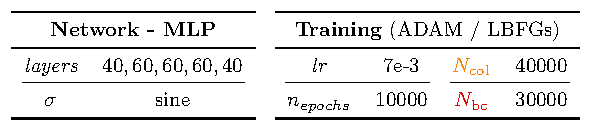
\includegraphics[width=0.94\linewidth]{images/appendix/training_param.pdf}
        \end{minipage}
        \begin{minipage}{0.36\linewidth}
            \centering
            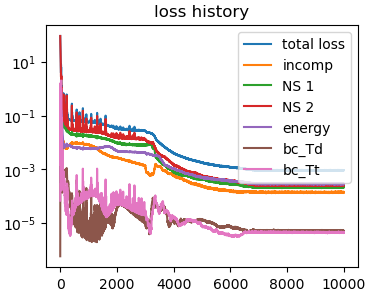
\includegraphics[width=0.84\linewidth]{images/appendix/test4_v5.png}
        \end{minipage}
    \end{center}
    
    \vspace{-8pt}
\end{appendixframe}

\begin{appendixframe}{Prediction on $\bm{\mu}^{(1)} = (0.1,0.1)$}
    \vspace{-4pt}
    \textbf{Prediction :} \begin{minipage}{0.26\linewidth}
        \centering
        $u_{1,\theta}$ \\
        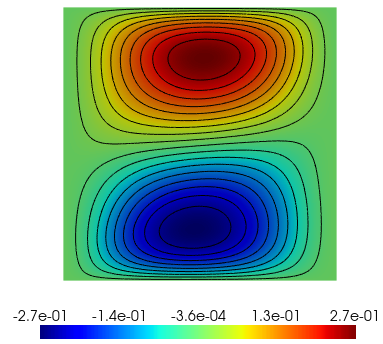
\includegraphics[width=0.95\linewidth]{images/appendix/PINN_plot_case4_v2_param1_u1.png}
    \end{minipage} \; \begin{minipage}{0.26\linewidth}
        \centering
        $u_{2,\theta}$ \\
        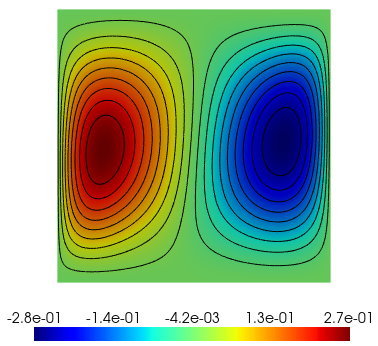
\includegraphics[width=0.95\linewidth]{images/appendix/PINN_plot_case4_v2_param1_u2.png}
    \end{minipage} \; \begin{minipage}{0.26\linewidth}
        \centering
        $T_\theta$ \\
        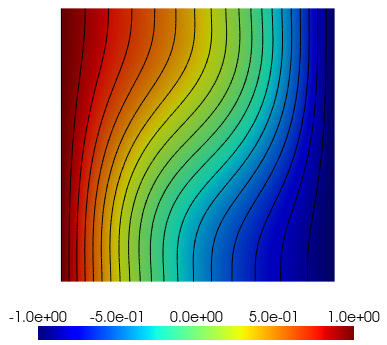
\includegraphics[width=0.95\linewidth]{images/appendix/PINN_plot_case4_v2_param1_T.png}
    \end{minipage}

    \vspace{8pt}

    \textbf{Error map :} \begin{minipage}{0.26\linewidth}
        \centering
        $u_{1,\text{ref}}-u_{1,\theta}$ \\
        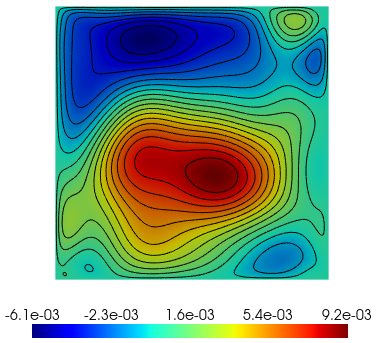
\includegraphics[width=0.95\linewidth]{images/appendix/PINN_error_plot_case4_v2_param1_u1.png}
    \end{minipage} \; \begin{minipage}{0.26\linewidth}
        \centering
        $u_{2,\text{ref}}-u_{2,\theta}$ \\
        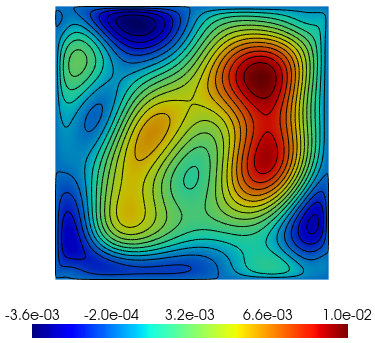
\includegraphics[width=0.95\linewidth]{images/appendix/PINN_error_plot_case4_v2_param1_u2.png}
    \end{minipage} \; \begin{minipage}{0.26\linewidth}
        \centering
        $T_\text{ref}-T_\theta$ \\
        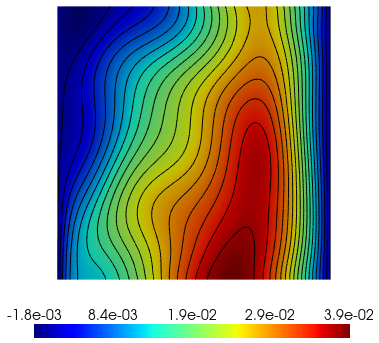
\includegraphics[width=0.95\linewidth]{images/appendix/PINN_error_plot_case4_v2_param1_T.png}
    \end{minipage}

    \vspace{8pt}

    \textbf{$L^2$ error :} \hspace{25pt} $2.98\times10^{-2} \hspace{42pt} 3.17\times10^{-2} \hspace{42pt}  3.90\times10^{-2}$

    \vspace{-2pt}
    \textbf{\small (relative)}
\end{appendixframe}

\appendixsubsection{Enriched FEM using PINN}

\begin{appendixframe}{Enriched space using PINN}
    Considering the PINN prior $U_\theta = (\bm{u}_\theta, p_\theta, T_\theta)$, we define the \textcolor{darkred}{mixed finite element space additively enriched} by the PINN as follows:
    
    \begin{center}
        \fcolorbox{darkred}{white}{$M_h^+ = \left\{U_h^+ = U_\theta + C_h^+, \quad C_h^+ \in M_h^{\, 0}\right\}$}
    \end{center}

    with $M_h^{\, 0}=[V_h^{\, 0}]^2 \times Q_h \times W_h^0$,
    $U_h^+ = (\bm{u}_h^+, p_h^+, T_h^+) \in M_h^+$ and $C_h^+ = (\bm{C}_{h,\bm{u}}^+, C_{h,p}^+, C_{h,T}^+)$.

    \vspace{8pt}

    We can then define the three finite element subspaces of $M_h^+$ as follows:
    \begin{minipage}{0.6\linewidth}
        \vspace{-15pt}
        \begin{align*}
            \bm{V}_h^+ &= \left\{\bm{u}_h^+ = \bm{u}_\theta + \bm{C}_{h,\bm{u}}^+, \; \bm{C}_{h,\bm{u}}^+ \in [V_h^{\, 0}]^2\right\}, \\
            Q_h^+ &= \left\{p_h^+ = p_\theta + C_{h,p}^+, \; C_{h,p}^+ \in Q_h\right\}, \\
            W_h^+ &= \left\{T_h^+ = T_\theta + C_{h,T}^+, \; C_{h,T}^+ \in W_h^{\, 0}\right\},
        \end{align*}
        where $\bm{C}_{h,\bm{u}}^+$, $C_{h,p}^+$ and $C_{h,T}^+$ becomes the unknowns.
        
        % \vspace{5pt}
        % \hl{à ajouter : dans quoi vit $U_\theta$ ?}
    \end{minipage}
    \begin{minipage}{0.38\linewidth}
        \centering
        \vspace{5pt}
        \pgfimage[width=0.7\linewidth]{images/appendix/correction.pdf}
    \end{minipage}
\end{appendixframe}

\begin{appendixframe}{Weak form - Additive approach}
    \textbf{Weak problem\myfootcite{Problem solved using Newton's algorithm with the correction vector initialized to $0$.} :} Find $C_h^+=(\textcolor{Cyan}{\bm{C}_{h,\bm{u}}^+}, \textcolor{blue}{C_{h,p}^+}, \textcolor{ForestGreen}{C_{h,T}^+}) \in M_h^{\, 0}$ s.t., \; $\forall (\bm{v}_h, q_h, w_h) \in M_h^{\, 0}$,

    \vspace{-4pt}
    \footnotesize
    \begin{equation}
        \label{eq:weak_pb_add}
        \hspace{-8pt}\begin{aligned}
            &\int_\Omega \big[(\textcolor{darkred}{\bm{u}_\theta} \cdot \nabla)\textcolor{darkred}{\bm{u}_\theta} + (\textcolor{darkred}{\bm{u}_\theta} \cdot \nabla)\textcolor{Cyan}{\bm{C}_{h,\bm{u}}^+} + (\textcolor{Cyan}{\bm{C}_{h,\bm{u}}^+} \cdot \nabla)\textcolor{darkred}{\bm{u}_\theta} + (\textcolor{Cyan}{\bm{C}_{h,\bm{u}}^+} \cdot \nabla)\textcolor{Cyan}{\bm{C}_{h,\bm{u}}^+} \big] \cdot \bm{v_h} \, d\bm{x} \\
            &\hspace{20pt} +\mu \left(\int_\Omega  \nabla \textcolor{darkred}{\bm{u}_\theta} : \nabla \bm{v}_h \, d\bm{x} + \int_\Omega \nabla \textcolor{Cyan}{\bm{C}_{h,\bm{u}}^+} : \nabla \bm{v}_h \, d\bm{x}\right) + \left(\int_\Omega \nabla \textcolor{darkred}{p_\theta} \cdot \bm{v}_h \, d\bm{x} - \int_\Omega \textcolor{blue}{C_{h,p}^+} \nabla \cdot \bm{v}_h \, d\bm{x}\right)\\
            &\hspace{50pt} - g \int_\Omega (1 + \beta (\textcolor{darkred}{T_\theta} + \textcolor{ForestGreen}{C_{h,T}^+})) \bm{e}_y \cdot \bm{v}_h \, d\bm{x} = 0, \,\text{\footnotesize (momentum)}  \\
            &\int_\Omega q_h \, \big[\nabla \cdot \textcolor{darkred}{\bm{u}_\theta} + \nabla \cdot \textcolor{Cyan}{\bm{C}_{h,\bm{u}}^+}\big] \, d\bm{x} \, + \, 10^{-4} \int_\Omega q_h \, (\textcolor{darkred}{p_\theta} + \textcolor{blue}{C_{h,p}^+}) \, d\bm{x} = 0, \; \text{\footnotesize (incompressibility + penal)} \\
            & \int_\Omega \big[ \textcolor{darkred}{\bm{u}_\theta} \cdot \nabla \textcolor{darkred}{T_\theta} + \textcolor{darkred}{\bm{u}_\theta} \cdot \nabla \textcolor{ForestGreen}{C_{h,T}^+} + \textcolor{Cyan}{\bm{C}_{h,\bm{u}}^+} \cdot \nabla \textcolor{darkred}{T_\theta} + \textcolor{Cyan}{\bm{C}_{h,\bm{u}}^+} \cdot \nabla \textcolor{ForestGreen}{C_{h,T}^+} \big] w_h \, d\bm{x} \\
            & \hspace{40pt} + k_f \left(\int_\Omega \nabla \textcolor{darkred}{T_\theta} \cdot \nabla w_h \; d\bm{x} + \int_\Omega \nabla \textcolor{ForestGreen}{C_{h,T}^+} \cdot \nabla w_h \, d\bm{x} \, w_h \, d\bm{s}\right) = 0, \, \text{\footnotesize (energy)}
        \end{aligned}
        \tag{$\mathcal{P}_h^+$}
    \end{equation}

    \vspace{5pt}
    with \textcolor{darkred}{$U_\theta = (\bm{u}_\theta, p_\theta, T_\theta)$} the PINN prior and some modified boundary conditions.
\end{appendixframe}

% \renewcommand{\insertsectionheadSubtitle}{
%     \begin{itemize}
%         \item Results obtained with a laptop GPU.
%         \item The newton solver is the same for all methods (rtol$=10^{-10}$, atol$=10^{-10}$, max\_it$=30$).
%         \item Additive approach : we consider $u_\theta$ in a $\mathbb{P}_3^2\times \mathbb{P}_2 \times \mathbb{P}_3$ continuous Lagrange FE space (defined on the current mesh).
%     \end{itemize}}
\appendixsubsection{Numerical results}

\begin{appendixframe}{Numerical costs}	
    $\bm{\mu}^{(1)}$ :

    \vspace{-20pt}
    \flushright
    
\includegraphics[width=0.9\linewidth]{images/appendix/cvg_param1.pdf}

    \flushleft
    % Defining the global error as the sum of the $L^2$ relatives errors on $\bm{u}$ and $T$.

    % \vspace{-5pt}
    $N_\text{dofs}$ and execution time required to reach the same global $L^2$ relative error $e$ :\myfootcite{Error defined as the sum of the $L^2$ relatives errors on $\bm{u}$ and $T$.}

    \begin{minipage}{0.32\linewidth}
        \centering
        % \qquad $\bm{\mu}^{(1)}=(0.1,0.1)$ \\
        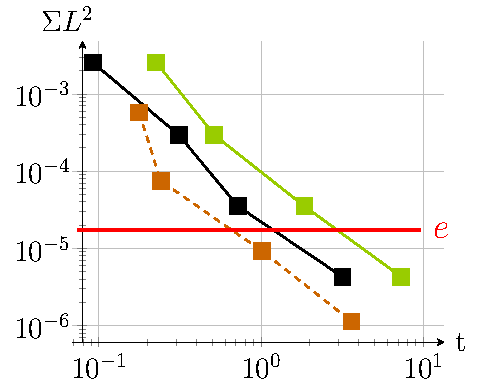
\includegraphics[width=0.9\linewidth]{images/appendix/time_param1_line.pdf}
    \end{minipage}
    \begin{minipage}{0.66\linewidth}
        \begin{tikzpicture}
            \node[anchor=south west, inner sep=0] (img) at (0,0) {
\includegraphics[height=2.4cm]{images/appendix/costs_param1.pdf}};
            \flechecourbe{2.5}{0.1}{1.4}{-0.1}{$\div 2.5$}
            \flechecourbe{6.3}{0.1}{1.2}{-0.1}{$\div 2$}
            \draw[thick,-,flechecolor]
            (5.3,0.1) .. controls (4.5+2.4,-0.3) and (4.5+2.4,-0.3) .. (7.5,0.1)
            node[midway, sloped, fill=white, inner sep=1pt] {\tiny $\div 4$};
        \end{tikzpicture}
    \end{minipage}

    \vspace{5pt}
\end{appendixframe}